% !TEX program = xelatex
% Bilingual (EN/中文) slides: Batched dense optical flow in PyTorch.
% Build:  cd slides && xelatex main.tex && xelatex main.tex
% (TeX Live 2018, no ctex/xeCJK on this machine -> fontspec + Droid Sans
%  Fallback + native XeTeX CJK line breaking; no pgfplots -> raw TikZ chart.)
\documentclass[aspectratio=169,10pt]{beamer}

\usepackage{fontspec}
\usepackage{amsmath,amssymb}
\usepackage{booktabs}
\usepackage{ifthen}
\usepackage{tikz}
\usetikzlibrary{positioning,calc,arrows.meta,decorations.pathreplacing}

% ---------- Chinese support (no ctex/xeCJK available on this TeX Live 2018) ----
\newfontfamily\zhfont{Droid Sans Fallback}
\XeTeXlinebreaklocale "zh"
\XeTeXlinebreakskip = 0pt plus 1pt
\newcommand{\zh}[1]{{\zhfont #1}}

% ---------- Colors (validated categorical palette) -----------------------------
\definecolor{cblue}{HTML}{2A78D6}   % backend: OpenCV CPU
\definecolor{corange}{HTML}{EB6834} % backend: OpenCV CUDA
\definecolor{caqua}{HTML}{1BAF7A}   % backend: Torch CPU
\definecolor{cyellow}{HTML}{EDA100} % backend: Torch CUDA
\definecolor{cred}{HTML}{E34948}
\definecolor{cink}{HTML}{0B0B0B}
\definecolor{cmut}{HTML}{52514E}

% ---------- Clean theme --------------------------------------------------------
\usetheme{default}
\setbeamertemplate{navigation symbols}{}
\setbeamertemplate{footline}{%
  \hfill{\scriptsize\color{cmut}\insertframenumber\,/\,\inserttotalframenumber}\hspace{2mm}\vspace{1mm}}
\setbeamercolor{frametitle}{fg=white,bg=cblue!85!black}
\setbeamerfont{frametitle}{series=\bfseries,size=\large}
\setbeamertemplate{frametitle}{%
  \nointerlineskip
  \begin{beamercolorbox}[wd=\paperwidth,sep=2.2mm]{frametitle}
    \insertframetitle
  \end{beamercolorbox}}
\setbeamercolor{title}{fg=cblue!70!black}
\setbeamercolor{structure}{fg=cblue}
\setbeamercolor{normal text}{fg=cink}
\setbeamertemplate{itemize items}{\textcolor{cblue}{\raisebox{.25ex}{\scriptsize$\blacktriangleright$}}}
\setbeamertemplate{itemize subitem}{\textcolor{caqua}{\raisebox{.25ex}{\scriptsize$\bullet$}}}

% Chinese summary box, one per slide, consistent style.
\setbeamercolor{cnbox}{bg=cblue!7,fg=cink}
\newenvironment{cn}{%
  \begin{beamercolorbox}[rounded=true,sep=4pt,wd=\textwidth]{cnbox}\zhfont\footnotesize
  {\color{cblue!70!black}\textbf{中文要点}}\quad}%
  {\end{beamercolorbox}}

% ==============================================================================
% RESULT PLACEHOLDERS -- fill pending numbers here (ONE edit point).
% Confirmed measurements (OpenCV CPU, 48-core login node):
\newcommand{\tvlCvCpuMs}{424}     % TV-L1  @240x320, ms/pair
\newcommand{\tvlCvCpuFps}{2.4}
\newcommand{\dfCvCpuMs}{346}      % DeepFlow @240x320, ms/pair
\newcommand{\dfCvCpuFps}{2.9}
\newcommand{\fbCvCpuMs}{84}       % Farneback @480x640, ms/pair
\newcommand{\tvlCvEpeGt}{0.149}   % TV-L1 EPE vs Middlebury GT
\newcommand{\dfCvEpeGt}{0.084}    % DeepFlow EPE vs Middlebury GT
% Pending (set the macro to the measured number; "TBD" renders as a gray
% placeholder in tables and as a dashed bar in the chart automatically):
\newcommand{\tvlCvCudaMs}{TBD}    % TV-L1  OpenCV CUDA, ms/pair
\newcommand{\tvlTorchCpuMs}{TBD}  % TV-L1  torch CPU,   ms/pair
\newcommand{\tvlTorchGpuMs}{TBD}  % TV-L1  torch CUDA (L40), ms/pair (batched)
\newcommand{\dfTorchCpuMs}{TBD}   % DeepFlow torch CPU, ms/pair
\newcommand{\dfTorchGpuMs}{TBD}   % DeepFlow torch CUDA (L40), ms/pair (batched)
\newcommand{\tvlTorchEpeGt}{TBD}  % TV-L1  torch EPE vs GT
\newcommand{\tvlTorchEpeCv}{TBD}  % TV-L1  torch EPE vs OpenCV reference
\newcommand{\dfTorchEpeGt}{TBD}   % DeepFlow torch EPE vs GT
\newcommand{\dfTorchEpeCv}{TBD}   % DeepFlow torch EPE vs OpenCV reference
% ==============================================================================

% "TBD" -> gray italic in tables; numbers pass through.
\newcommand{\pend}[1]{\ifthenelse{\equal{#1}{TBD}}{{\color{cmut}\itshape TBD}}{#1}}

% Bar for the runtime chart: #1 x-center, #2 value macro (ms or TBD), #3 color.
% Scale: 1 cm = 100 ms.
\newcommand{\benchbar}[3]{%
  \ifthenelse{\equal{#2}{TBD}}{%
    \draw[dashed,#3,thick,fill=#3!10] (#1-0.3,0) rectangle (#1+0.3,0.9);
    \node[above] at (#1,0.9) {\scriptsize\color{cmut}TBD};
  }{%
    \pgfmathsetmacro{\bh}{#2/100}%
    \fill[#3,rounded corners=1.5pt] (#1-0.3,0) rectangle (#1+0.3,\bh);
    \node[above] at (#1,\bh) {\scriptsize #2};
  }}

\title{Batched Dense Optical Flow in PyTorch\\[1ex]
  {\zhfont\large 批量稠密光流的 PyTorch 实现与基准测试}}
\subtitle{TV-L1 \& DeepFlow: OpenCV CPU vs.\ CUDA vs.\ pure-torch reimplementation}
\author{T.~Long \\ {\footnotesize tlong32@jhu.edu}}
\date{August 2026}

\begin{document}

% ---------------------------------------------------------------- 1 title -----
\begin{frame}[plain]
  \titlepage
  \vfill
  \centering\scriptsize\color{cmut}
  Middlebury pairs $480\times640$ \quad$\cdot$\quad NVIDIA L40 (SLURM, ilps-cn119)
  \quad$\cdot$\quad 48-core CPU login node
\end{frame}

% ------------------------------------------------------------- 2 motivation ---
\begin{frame}{Motivation \zh{研究动机}}
  \begin{itemize}
    \item Dense optical flow is a standard \textbf{preprocessing step at scale}:
      video understanding, motion features, temporal augmentation, dataset
      curation --- millions of frame pairs, not one.
    \item Classic accurate methods (TV-L1, DeepFlow) are \textbf{variational}:
      hundreds of small iterations per pair $\Rightarrow$ slow on CPU,
      awkward on GPU.
    \item What matters for preprocessing is \textbf{batch throughput}
      (pairs/second over a whole dataset), not single-pair latency.
    \item Goal: benchmark OpenCV CPU vs.\ OpenCV CUDA vs.\ our
      \textbf{batched pure-PyTorch reimplementations}, on identical inputs and
      parameters.
  \end{itemize}
  \vfill
  \begin{cn}
    稠密光流常作为大规模视频处理的预处理步骤：要处理的是数百万帧对，而非单帧。
    经典变分方法（TV-L1、DeepFlow）迭代次数多、单对速度慢；预处理场景真正重要的是
    \textbf{批量吞吐量}。我们在相同输入与参数下对比 OpenCV CPU / OpenCV CUDA /
    自研批量化 PyTorch 实现。
  \end{cn}
\end{frame}

% ----------------------------------------------------------------- 3 setup ----
\begin{frame}{Benchmark Setup \zh{实验设置}}
  \begin{columns}[T]
    \begin{column}{0.56\textwidth}
      \textbf{Data \& hardware}
      \begin{itemize}
        \item Middlebury training pairs, $480\times640$ grayscale
          (also downscaled $240\times320$); ground-truth flow for EPE.
        \item GPU: NVIDIA L40 (142 SMs), SLURM node \texttt{ilps-cn119}.
        \item CPU: 48-core login node.
        \item Env: \texttt{uv}-managed;
          \texttt{opencv-contrib-python-headless}, PyTorch.
      \end{itemize}
    \end{column}
    \begin{column}{0.42\textwidth}
      \textbf{Algorithm $\times$ backend matrix}
      {\small
      \begin{tabular}{@{}lccc@{}}
        \toprule
                 & cv CPU & cv CUDA & torch \\
        \midrule
        TV-L1    & \checkmark & \checkmark$^{*}$ & \checkmark \\
        DeepFlow & \checkmark & \textcolor{cred}{none} & \checkmark \\
        Farneback& \checkmark & \checkmark$^{*}$ & --- \\
        \bottomrule
      \end{tabular}}
      \par\smallskip
      {\scriptsize $^{*}$only with a custom CUDA build of OpenCV ---
        pip wheels ship \textbf{without} CUDA.}
    \end{column}
  \end{columns}
  \vfill
  \begin{cn}
    数据：Middlebury 训练集（$480\times640$，含真值光流，用于计算端点误差 EPE）。
    硬件：NVIDIA L40（142 个 SM，SLURM 节点）对比 48 核 CPU 登录节点。
    注意：pip 安装的 OpenCV 不带 CUDA，需要自行编译；DeepFlow 在 OpenCV 中
    \textbf{没有任何 CUDA 版本}。
  \end{cn}
\end{frame}

% ------------------------------------------------------------ 4 tvl1 energy ---
\begin{frame}{TV-L1: Energy Formulation \zh{能量泛函}}
  {\small (Zach, Pock, Bischof 2007) Total-variation regularizer + robust $L^1$ data term:}
  \begin{equation*}
    E(\mathbf{u}) \;=\; \int_{\Omega}
      \lambda\,\bigl|\rho(\mathbf{u}(\mathbf{x}))\bigr|
      \;+\; |\nabla u_1| + |\nabla u_2| \;\, d\mathbf{x}
  \end{equation*}
  with the image residual linearized around the current warp $\mathbf{u}^0$:
  \begin{equation*}
    \rho(\mathbf{u}) \;=\; I_1(\mathbf{x}+\mathbf{u}^0)
      \;+\; \bigl\langle \nabla I_1(\mathbf{x}+\mathbf{u}^0),\,
            \mathbf{u}-\mathbf{u}^0 \bigr\rangle \;-\; I_0(\mathbf{x})
  \end{equation*}
  \begin{itemize}
    \item $L^1$ data term: robust to outliers/occlusions; TV term: allows sharp
      flow discontinuities at motion boundaries.
    \item Both terms non-smooth $\Rightarrow$ solved via \textbf{duality}, not
      gradient descent.
    \item Params used (OpenCV defaults): $\lambda=0.15$, $\theta=0.3$,
      $\tau=0.25$, 5 scales (step $0.8$), 5 warps, up to $10\times30$
      primal--dual iterations.
  \end{itemize}
  \vfill
  \begin{cn}
    能量 = 全变差正则项 + 鲁棒 $L^1$ 数据项；$\rho$ 是在当前解 $\mathbf{u}^0$
    处线性化的亮度残差。$L^1$ 对遮挡/离群点鲁棒，TV 项保留运动边界的不连续性。
    两项都不可微，因此用\textbf{对偶方法}求解而非梯度下降。
  \end{cn}
\end{frame}

% ----------------------------------------------------------- 5 tvl1 duality ---
\begin{frame}{TV-L1: Duality Splitting \& Iterations \zh{对偶分裂与迭代}}
  Auxiliary field $\mathbf{v}$ decouples the two terms ($\theta$-coupling):
  \begin{equation*}
    \min_{\mathbf{u},\mathbf{v}} \int_{\Omega}
      |\nabla u_1| + |\nabla u_2|
      + \tfrac{1}{2\theta}\,\|\mathbf{u}-\mathbf{v}\|^2
      + \lambda\,|\rho(\mathbf{v})| \; d\mathbf{x}
  \end{equation*}
  \textbf{1) Pointwise thresholding} (closed form in $\mathbf{v}$):
  \begin{equation*}
    \mathbf{v} = \mathbf{u} +
    \begin{cases}
      \lambda\theta\,\nabla I_1 & \text{if } \rho(\mathbf{u}) < -\lambda\theta\,|\nabla I_1|^2\\
      -\lambda\theta\,\nabla I_1 & \text{if } \rho(\mathbf{u}) > \lambda\theta\,|\nabla I_1|^2\\
      -\rho(\mathbf{u})\,\nabla I_1 / |\nabla I_1|^2 & \text{if } |\rho(\mathbf{u})| \le \lambda\theta\,|\nabla I_1|^2
    \end{cases}
  \end{equation*}
  \textbf{2) TV proximal step} via dual variables $\mathbf{p}_d$ (Chambolle),
  for $d=1,2$:
  \begin{equation*}
    u_d = v_d + \theta\,\mathrm{div}\,\mathbf{p}_d, \qquad
    \mathbf{p}_d^{\,n+1} =
      \frac{\mathbf{p}_d^{\,n} + \tfrac{\tau}{\theta}\nabla u_d^{\,n+1}}
           {1 + \tfrac{\tau}{\theta}\bigl|\nabla u_d^{\,n+1}\bigr|}
    \quad (\text{projection onto } |\mathbf{p}_d|\le 1),\; \tau \le 1/4
  \end{equation*}
  \begin{cn}
    引入辅助变量 $\mathbf{v}$ 将两项解耦：第一步对每个像素做\textbf{闭式阈值化}
    更新 $\mathbf{v}$；第二步用对偶变量 $\mathbf{p}$ 做 TV 近端步
    （分母即到单位球的投影）。两步都是\textbf{纯逐像素运算}——非常适合张量化。
  \end{cn}
\end{frame}

% ---------------------------------------------------------- 6 pyramid tikz ----
\begin{frame}{Coarse-to-Fine Pyramid + Warping \zh{由粗到细金字塔与图像变形}}
  \centering
  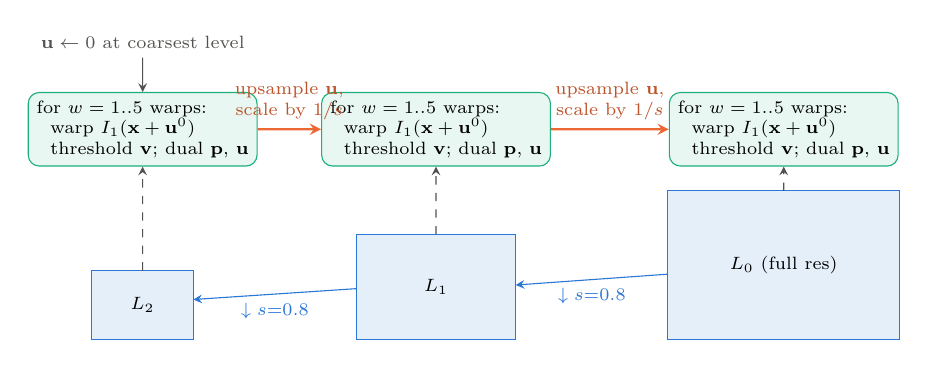
\begin{tikzpicture}[>=stealth,scale=0.92,every node/.style={transform shape}]
    % image pyramid levels
    \draw[fill=cblue!12,draw=cblue] (0.35,0)   rectangle (1.75,0.95) node[midway]{\scriptsize $L_2$};
    \draw[fill=cblue!12,draw=cblue] (4.0,0)  rectangle (6.2,1.45) node[midway]{\scriptsize $L_1$};
    \draw[fill=cblue!12,draw=cblue] (8.3,0)  rectangle (11.5,2.05) node[midway]{\scriptsize $L_0$ (full res)};
    % solver boxes above
    \node[draw=caqua,fill=caqua!10,rounded corners,align=left,font=\scriptsize]
      (s2) at (1.05,2.9) {for $w=1..5$ warps:\\ \ \ warp $I_1(\mathbf{x}+\mathbf{u}^0)$\\ \ \ threshold $\mathbf{v}$; dual $\mathbf{p}$, $\mathbf{u}$};
    \node[draw=caqua,fill=caqua!10,rounded corners,align=left,font=\scriptsize]
      (s1) at (5.1,2.9) {for $w=1..5$ warps:\\ \ \ warp $I_1(\mathbf{x}+\mathbf{u}^0)$\\ \ \ threshold $\mathbf{v}$; dual $\mathbf{p}$, $\mathbf{u}$};
    \node[draw=caqua,fill=caqua!10,rounded corners,align=left,font=\scriptsize]
      (s0) at (9.9,2.9) {for $w=1..5$ warps:\\ \ \ warp $I_1(\mathbf{x}+\mathbf{u}^0)$\\ \ \ threshold $\mathbf{v}$; dual $\mathbf{p}$, $\mathbf{u}$};
    % init and upsample arrows
    \node[font=\scriptsize,color=cmut] (init) at (1.05,4.1) {$\mathbf{u}\leftarrow 0$ at coarsest level};
    \draw[->,cmut] (init) -- (s2);
    \draw[->,thick,corange] (s2) -- (s1)
      node[midway,above,font=\scriptsize,align=center,color=corange!80!black]{upsample $\mathbf{u}$,\\ scale by $1/s$};
    \draw[->,thick,corange] (s1) -- (s0)
      node[midway,above,font=\scriptsize,align=center,color=corange!80!black]{upsample $\mathbf{u}$,\\ scale by $1/s$};
    % downsample arrows between images
    \draw[->,cblue] (4.0,0.7) -- (1.75,0.55) node[midway,below,font=\scriptsize,color=cblue]{$\downarrow s{=}0.8$};
    \draw[->,cblue] (8.3,0.9) -- (6.2,0.75) node[midway,below,font=\scriptsize,color=cblue]{$\downarrow s{=}0.8$};
    % level -> solver
    \draw[->,cmut,dashed] (1.05,0.95) -- (s2);
    \draw[->,cmut,dashed] (5.1,1.45) -- (s1);
    \draw[->,cmut,dashed] (9.9,2.05) -- (s0);
  \end{tikzpicture}
  \par\smallskip
  {\small Linearization $\rho$ is only valid for \emph{small} displacements
  $\Rightarrow$ estimate coarse motion on small images, then warp $I_1$ by the
  upsampled flow and re-linearize at each finer level.}
  \vfill
  \begin{cn}
    线性化残差 $\rho$ 只对小位移成立：先在低分辨率估计大运动，再逐层上采样光流
    （数值乘 $1/s$），用它对 $I_1$ 做 warp 后重新线性化。每层做 5 次 warp，
    每次 warp 内做数百次原始-对偶迭代。
  \end{cn}
\end{frame}

% ------------------------------------------------------------ 7 deepflow ------
\begin{frame}{DeepFlow: Variational Energy \zh{变分能量}}
  {\small (Weinzaepfel et al., ICCV 2013) --- Brox-style energy; robust penalty
   $\Psi(s^2)=\sqrt{s^2+\varepsilon^2}$, $\varepsilon=10^{-3}$:}
  \begin{align*}
    E(\mathbf{w}) \;=\; \int_{\Omega} \Bigl[\;
        &\delta\, \Psi\!\bigl(|I_2(\mathbf{x}+\mathbf{w})-I_1(\mathbf{x})|^2\bigr)
        && \text{\footnotesize brightness constancy}\\[-2pt]
      +\;&\gamma\, \Psi\!\bigl(\|\nabla I_2(\mathbf{x}+\mathbf{w})-\nabla I_1(\mathbf{x})\|^2\bigr)
        && \text{\footnotesize gradient constancy}\\[-2pt]
      +\;&\alpha\, \Psi\!\bigl(\|\nabla u\|^2+\|\nabla v\|^2\bigr)
        \;\Bigr]\, d\mathbf{x}
        && \text{\footnotesize smoothness}
  \end{align*}
  \begin{itemize}
    \item Full DeepFlow adds a matching term
      $\beta\, E_{\mathrm{match}}$ driving the flow toward
      \textbf{DeepMatching} correspondences.
    \item \textbf{OpenCV's \texttt{createOptFlow\_DeepFlow} implements only the
      variational part} --- no DeepMatching ($\beta=0$).
    \item Params (OpenCV defaults): $\alpha=1$, $\delta=0.5$, $\gamma=5$,
      pyramid downscale $0.95$ ($\sim$40+ levels), 5 fixed-point iterations,
      25 SOR iterations, $\omega=1.6$.
  \end{itemize}
  \vfill
  \begin{cn}
    能量含亮度守恒（权重 $\delta$）、梯度守恒（$\gamma$）与平滑项（$\alpha$），
    均用鲁棒罚函数 $\Psi(s^2)=\sqrt{s^2+\varepsilon^2}$。完整 DeepFlow 另有
    DeepMatching 匹配项；\textbf{OpenCV 只实现了变分部分}（无匹配项）。
  \end{cn}
\end{frame}

% -------------------------------------------------- 8 deepflow solver + rb ----
\begin{frame}{DeepFlow: Fixed-Point + Red-Black SOR \zh{不动点迭代与红黑 SOR}}
  \begin{columns}[T]
    \begin{column}{0.58\textwidth}
      \begin{itemize}\itemsep1pt
        \item Euler--Lagrange equations are nonlinear in
          $\mathbf{w}=(u,v)$: \textbf{fixed-point linearization} --- freeze
          $\Psi'$ weights and image derivatives at $\mathbf{w}^k$, solve for
          the increment $d\mathbf{w}$.
        \item Each linearization yields a large \textbf{sparse linear system}
          (5-point stencil per pixel, $2$ coupled channels).
        \item Solved by \textbf{SOR} ($\omega=1.6$): each pixel update mixes its
          own residual with already-updated neighbors.
        \item \textbf{Red-black ordering}: a red pixel's stencil touches only
          black pixels, so \emph{all red pixels update simultaneously}, then
          all black --- two fully parallel half-sweeps.
      \end{itemize}
    \end{column}
    \begin{column}{0.40\textwidth}
      \centering
      
\begin{tikzpicture}[scale=0.55,>=stealth]
        \foreach \i in {0,...,5}{\foreach \j in {0,...,5}{
          \pgfmathparse{mod(\i+\j,2)}
          \ifdim\pgfmathresult pt=0pt
            \fill[cred!85] (\i,\j) rectangle ++(1,1);
          \else
            \fill[cink!80] (\i,\j) rectangle ++(1,1);
          \fi}}
        \draw[white,line width=0.8pt] (0,0) grid (6,6);
        % arrows: red cell (2,3)..(3,4) center -> 4 black neighbors
        \draw[->,white,ultra thick] (2.5,3.5) -- (1.7,3.5);
        \draw[->,white,ultra thick] (2.5,3.5) -- (3.3,3.5);
        \draw[->,white,ultra thick] (2.5,3.5) -- (2.5,2.7);
        \draw[->,white,ultra thick] (2.5,3.5) -- (2.5,4.3);
      \end{tikzpicture}
      \par{\scriptsize A \textcolor{cred!85}{red} update reads only
        \textbf{black} neighbors $\Rightarrow$ each half-sweep is one
        \emph{vectorized masked update}.}
    \end{column}
  \end{columns}
  \vfill
  \begin{cn}
    外层\textbf{不动点迭代}固定 $\Psi'$ 权重得到稀疏线性方程组，内层用
    SOR（$\omega=1.6$）求解；\textbf{红黑排序}下红格只依赖黑格，
    红/黑各自可全并行更新——即两次带掩码的张量化更新。
  \end{cn}
\end{frame}

% -------------------------------------------------------- 9 why cv gpu bad ----
\begin{frame}{Why OpenCV GPU Is Limited Here \zh{OpenCV GPU 路线的局限}}
  \begin{enumerate}\itemsep3pt
    \item \textbf{Packaging}: pip \texttt{opencv-python} wheels ship
      \emph{without} CUDA $\Rightarrow$ custom source build per
      cluster/CUDA version --- a real operational burden.
    \item \textbf{API is one-pair-at-a-time}: \texttt{cv2.cuda} takes a single
      \texttt{GpuMat} pair. A $480{\times}640$ (let alone $240{\times}320$)
      problem cannot fill an L40's \textbf{142 SMs}; upload/download +
      kernel-launch overhead dominates.
    \item \textbf{Hundreds of tiny sequential iterations}: TV-L1 $\approx$
      5 scales $\times$ 5 warps $\times$ up to 300 primal--dual steps
      $\Rightarrow$ thousands of small kernels per pair --- \emph{launch-bound},
      GPU mostly idle.
    \item \textbf{DeepFlow: no CUDA version exists in OpenCV at all}; and a
      naive (lexicographic) SOR sweep is inherently sequential --- it must be
      re-ordered (red-black) to parallelize.
  \end{enumerate}
  \vfill
  \begin{cn}
    （1）pip 版 OpenCV 不含 CUDA，须自行编译；（2）\texttt{cv2.cuda} 一次只处理
    一对图像，小图无法喂饱 L40 的 142 个 SM，上传/下载与核启动开销占主导；
    （3）TV-L1 有成千上万个微小串行核，属于\textbf{启动开销受限}；
    （4）DeepFlow 根本没有 OpenCV CUDA 版本，且朴素 SOR 天生串行。
  \end{cn}
\end{frame}

% -------------------------------------------------------- 10 timeline tikz ----
\begin{frame}{Launch-Bound vs.\ Batched \zh{核启动受限 vs.\ 批量化}}
  \centering
  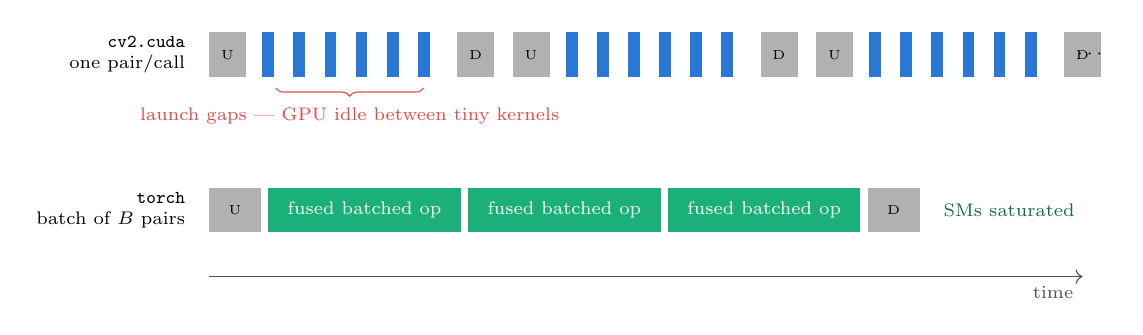
\begin{tikzpicture}[scale=0.94,font=\scriptsize,every node/.style={transform shape}]
    % ---- top track: cv2.cuda one pair per call
    \node[anchor=east,align=right] at (-0.2,3.1) {\texttt{cv2.cuda}\\one pair/call};
    \foreach \o in {0,4.1,8.2}{
      \fill[cmut!45] (\o,2.8) rectangle ++(0.5,0.6);
      \node at (\o+0.25,3.1) {\tiny U};
      \foreach \k in {0,1,...,5}{
        \fill[cblue] (\o+0.72+\k*0.42,2.8) rectangle ++(0.16,0.6);}
      \fill[cmut!45] (\o+3.35,2.8) rectangle ++(0.5,0.6);
      \node at (\o+3.6,3.1) {\tiny D};}
    \node[anchor=west] at (11.6,3.1) {$\cdots$};
    \draw[decorate,decoration={brace,mirror,amplitude=3pt},cred]
      (0.9,2.65) -- (2.9,2.65) node[midway,below=4pt,color=cred]
      {launch gaps --- GPU idle between tiny kernels};
    % ---- bottom track: torch batched
    \node[anchor=east,align=right] at (-0.2,1.0) {\texttt{torch}\\batch of $B$ pairs};
    \fill[cmut!45] (0,0.7) rectangle ++(0.7,0.6); \node at (0.35,1.0) {\tiny U};
    \fill[caqua] (0.8,0.7) rectangle ++(2.6,0.6);
    \fill[caqua] (3.5,0.7) rectangle ++(2.6,0.6);
    \fill[caqua] (6.2,0.7) rectangle ++(2.6,0.6);
    \node[color=white] at (2.1,1.0) {fused batched op};
    \node[color=white] at (4.8,1.0) {fused batched op};
    \node[color=white] at (7.5,1.0) {fused batched op};
    \fill[cmut!45] (8.9,0.7) rectangle ++(0.7,0.6); \node at (9.25,1.0) {\tiny D};
    \node[anchor=west,color=caqua!60!black] at (9.8,1.0) {SMs saturated};
    % time axis
    \draw[->,cmut] (0,0.1) -- (11.8,0.1) node[below left]{time};
  \end{tikzpicture}
  \par\bigskip
  {\small Same total math --- but one launch now covers $B$ images' worth of
  pixels, so arithmetic hides the launch latency and fills the GPU.}
  \vfill
  \begin{cn}
    上：\texttt{cv2.cuda} 每对图像触发一串微小核函数，核间空隙里 GPU 空转。
    下：批量张量把 $B$ 对图像合成一次大核启动——总计算量相同，但每次启动的
    工作量足以摊薄启动延迟并填满所有 SM。
  \end{cn}
\end{frame}

% ---------------------------------------------------------- 11 our approach ---
\begin{frame}{Our Approach: Pure-Torch, Batched \zh{纯 PyTorch 批量化实现}}
  \texttt{torch\_flow.py} (\texttt{calc\_flow\_tvl1}) \quad$\cdot$\quad
  \texttt{torch\_deepflow.py} (\texttt{calc\_flow\_deepflow})
  \begin{itemize}\itemsep2pt
    \item \textbf{Batched end to end}: $(B,H,W)$ image pairs $\to$
      $(B,2,H,W)$ flows; every step is a vectorized tensor op over the whole
      batch --- no Python loop over pairs.
    \item \textbf{Warping} = \texttt{grid\_sample} (bilinear, one call for the
      batch).
    \item \textbf{Red-black SOR / primal--dual} steps as masked tensor
      updates: two half-sweeps $=$ two fused elementwise ops.
    \item \textbf{Same code on CPU and CUDA} --- just
      \texttt{.to(device)}; no custom OpenCV build.
    \item \textbf{Composable} with a torch pipeline: \texttt{DataLoader}
      feeding, \texttt{torch.no\_grad()} inference,
      \texttt{torch.compile} for kernel fusion.
  \end{itemize}
  \vfill
  \begin{cn}
    输入 $(B,H,W)$ 帧对、输出 $(B,2,H,W)$ 光流，全流程张量化：warp 用
    \texttt{grid\_sample}，红黑 SOR / 原始-对偶迭代化为带掩码的融合逐元素运算。
    同一份代码在 CPU 与 GPU 上直接运行，且天然融入 torch 数据管线
    （DataLoader、\texttt{no\_grad} 推理、\texttt{torch.compile}）。
  \end{cn}
\end{frame}

% ------------------------------------------------------- 12 runtime table -----
\begin{frame}{Runtime Results \zh{运行时间结果}}
  \centering
  {\small Per-pair wall time, identical parameters across backends.
   \textcolor{cmut}{\itshape TBD} = measurement in progress.}
  \par\medskip
  \begin{tabular}{@{}llrrrr@{}}
    \toprule
    Algorithm & Size & \textcolor{cblue}{cv CPU} & \textcolor{corange}{cv CUDA}
      & \textcolor{caqua!70!black}{torch CPU} & \textcolor{cyellow!70!black}{torch CUDA (L40)} \\
    \midrule
    TV-L1    & $240{\times}320$ & \tvlCvCpuMs\,ms (\tvlCvCpuFps\,FPS)
             & \pend{\tvlCvCudaMs} & \pend{\tvlTorchCpuMs} & \pend{\tvlTorchGpuMs} \\
    DeepFlow & $240{\times}320$ & \dfCvCpuMs\,ms (\dfCvCpuFps\,FPS)
             & --- (none) & \pend{\dfTorchCpuMs} & \pend{\dfTorchGpuMs} \\
    Farneback & $480{\times}640$ & \fbCvCpuMs\,ms & --- & --- & --- \\
    \bottomrule
  \end{tabular}
  \par\medskip
  \begin{itemize}
    \item CPU numbers from the 48-core login node --- but these algorithms
      \textbf{barely parallelize} in OpenCV: Farneback single-thread vs
      48-thread is 85 vs 84\,ms. Cores don't help; batching must.
    \item torch CUDA column is \textbf{batched} throughput
      (time per pair $=$ batch time $/ B$).
  \end{itemize}
  \vfill
  \begin{cn}
    OpenCV CPU 已确认：TV-L1 每对 424 毫秒、DeepFlow 346 毫秒（$240\times320$）。
    48 核几乎不加速（Farneback 单线程 85 ms vs 48 线程 84 ms）——多核帮不上忙，
    必须靠批量化。torch CPU/GPU 数据测量中（表中 TBD 一处修改即可全局填入）。
  \end{cn}
\end{frame}

% -------------------------------------------------------- 13 bar chart --------
\begin{frame}{Runtime Chart \zh{运行时间对比图}}
  \centering
  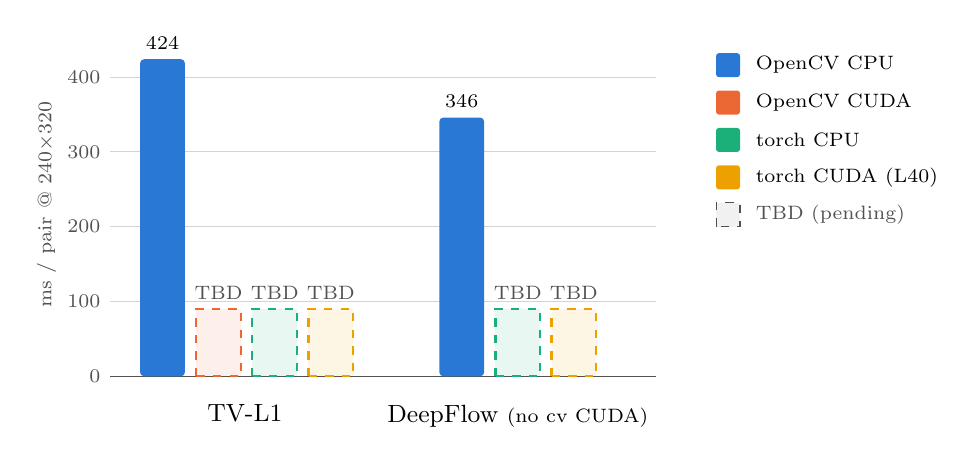
\begin{tikzpicture}[scale=0.95]
    % axis + grid (1 cm = 100 ms)
    \foreach \y in {1,2,3,4}{
      \draw[cmut!25] (0.3,\y) -- (7.6,\y);
      \node[left,font=\scriptsize,color=cmut] at (0.3,\y) {\y00};}
    \node[left,font=\scriptsize,color=cmut] at (0.3,0) {0};
    \draw[cmut] (0.3,0) -- (7.6,0);
    \node[rotate=90,font=\scriptsize,color=cmut] at (-0.55,2.3) {ms / pair @ $240{\times}320$};
    % TV-L1 group
    \benchbar{1.0}{\tvlCvCpuMs}{cblue}
    \benchbar{1.75}{\tvlCvCudaMs}{corange}
    \benchbar{2.5}{\tvlTorchCpuMs}{caqua}
    \benchbar{3.25}{\tvlTorchGpuMs}{cyellow}
    \node[below,font=\small] at (2.1,-0.25) {TV-L1};
    % DeepFlow group (no cv CUDA)
    \benchbar{5.0}{\dfCvCpuMs}{cblue}
    \benchbar{5.75}{\dfTorchCpuMs}{caqua}
    \benchbar{6.5}{\dfTorchGpuMs}{cyellow}
    \node[below,font=\small] at (5.75,-0.25) {DeepFlow \scriptsize(no cv CUDA)};
    % legend
    \begin{scope}[shift={(8.4,2.4)}]
      \foreach \c/\t/\yy in {cblue/OpenCV CPU/1.6, corange/OpenCV CUDA/1.1,
                             caqua/torch CPU/0.6, cyellow/torch CUDA (L40)/0.1}{
        \fill[\c,rounded corners=1pt] (0,\yy) rectangle ++(0.32,0.32);
        \node[right,font=\scriptsize] at (0.4,\yy+0.16) {\t};}
      \draw[dashed,cmut,fill=cmut!8] (0,-0.4) rectangle ++(0.32,0.32);
      \node[right,font=\scriptsize,color=cmut] at (0.4,-0.24) {TBD (pending)};
    \end{scope}
  \end{tikzpicture}
  \par\smallskip
  {\scriptsize Dashed bars: measurements pending; heights will update
  automatically from the placeholder macros.}
  \vfill
  \begin{cn}
    实心柱为已确认的 OpenCV CPU 结果；虚线柱为待测的 torch CPU / torch CUDA
    与 OpenCV CUDA 结果，数值填入宏后柱高自动更新。
  \end{cn}
\end{frame}

% ---------------------------------------------------------- 14 accuracy -------
\begin{frame}{Accuracy: Endpoint Error \zh{精度：端点误差}}
  \centering
  {\small Mean EPE on Middlebury pairs at $240{\times}320$
   (pixels with GT magnitude $>10^9$, i.e.\ ``unknown'', excluded).}
  \par\medskip
  \begin{tabular}{@{}llccc@{}}
    \toprule
    Algorithm & Backend & EPE vs.\ GT & EPE vs.\ OpenCV ref. \\
    \midrule
    TV-L1    & OpenCV CPU & \tvlCvEpeGt & (reference) \\
    TV-L1    & torch      & \pend{\tvlTorchEpeGt} & \pend{\tvlTorchEpeCv} \\
    \midrule
    DeepFlow & OpenCV CPU & \dfCvEpeGt & (reference) \\
    DeepFlow & torch      & \pend{\dfTorchEpeGt} & \pend{\dfTorchEpeCv} \\
    \bottomrule
  \end{tabular}
  \par\medskip
  \begin{itemize}
    \item DeepFlow's variational part is already notably more accurate than
      TV-L1 here (0.084 vs 0.149 EPE).
    \item ``EPE vs.\ OpenCV ref.''\ measures \textbf{faithfulness of the
      reimplementation} (target $\ll$ EPE vs.\ GT); small differences expected
      from interpolation/boundary choices.
  \end{itemize}
  \vfill
  \begin{cn}
    以 Middlebury 真值计算平均端点误差（EPE）：DeepFlow（0.084）明显优于
    TV-L1（0.149）。“vs.\ OpenCV”一列衡量我们复现实现与 OpenCV 的一致性，
    目标是远小于对真值的误差；插值与边界处理会带来微小差异。torch 数据待填。
  \end{cn}
\end{frame}

% -------------------------------------------------------- 15 conclusions ------
\begin{frame}{Conclusions \& Practical Notes \zh{结论与实用备注}}
  \textbf{Conclusions}
  \begin{itemize}\itemsep1pt
    \item Variational flow is iteration-heavy and core-count-insensitive; the
      viable route to throughput is \textbf{batching}, which OpenCV's APIs
      (CPU or CUDA) do not offer.
    \item A pure-torch rewrite gives batching, GPU support without custom
      OpenCV builds, one code path for CPU/GPU, and pipeline composability.
    \item Red-black reordering is the key trick that makes SOR-style solvers
      tensor-friendly.
  \end{itemize}
  \smallskip
  \textbf{Practical notes}
  \begin{itemize}\itemsep1pt
    \item Env: \texttt{uv} project; use
      \texttt{opencv-contrib-python-headless} on compute nodes (no GUI libs).
    \item GPU runs via SLURM: {\footnotesize
      \texttt{srun -p gpu -w ilps-cn119 --gres=gpu:1 --cpus-per-task=8
      --mem=16G uv run --no-sync python benchmark.py}}
    \item Login node has no GPU: CPU backends only; benchmark script
      auto-skips unavailable backends.
  \end{itemize}
  \vfill
  \begin{cn}
    结论：变分光流迭代多、对核数不敏感，吞吐量的正确路径是\textbf{批量化}；
    纯 torch 重写免去 OpenCV 自编译、CPU/GPU 一套代码、可组合进现有管线。
    实用：用 \texttt{uv} 管理环境，计算节点装 headless 版 OpenCV，GPU 作业经
    SLURM 提交至 ilps-cn119。
  \end{cn}
\end{frame}

% ---------------------------------------------------------- 16 references -----
\begin{frame}{References \zh{参考文献}}
  \small
  \begin{enumerate}\itemsep4pt
    \item C.~Zach, T.~Pock, H.~Bischof.
      \emph{A Duality Based Approach for Realtime TV-L1 Optical Flow.}
      DAGM Symposium on Pattern Recognition, 2007.
    \item P.~Weinzaepfel, J.~Revaud, Z.~Harchaoui, C.~Schmid.
      \emph{DeepFlow: Large Displacement Optical Flow with Deep Matching.}
      ICCV 2013.
    \item J.~S\'anchez~P\'erez, E.~Meinhardt-Llopis, G.~Facciolo.
      \emph{TV-L1 Optical Flow Estimation.}
      Image Processing On Line (IPOL), vol.~3, 2013.
    \item S.~Baker, D.~Scharstein, J.P.~Lewis, S.~Roth, M.J.~Black, R.~Szeliski.
      \emph{A Database and Evaluation Methodology for Optical Flow.}
      IJCV, 2011. (Middlebury benchmark)
    \item OpenCV documentation:
      \texttt{cv::optflow::DualTVL1OpticalFlow},
      \texttt{cv::optflow::createOptFlow\_DeepFlow},
      \texttt{cv::cuda::OpticalFlowDual\_TVL1}.
  \end{enumerate}
  \vfill
  \begin{cn}
    以上为 TV-L1（Zach 等 2007；S\'anchez 等 IPOL 2013 实现）、DeepFlow
    （Weinzaepfel 等 ICCV 2013）、Middlebury 数据集及 OpenCV 文档的出处。
  \end{cn}
\end{frame}

\end{document}
